\documentclass[12pt,a4paper]{extreport}
\usepackage[T1]{fontenc}
\usepackage[french]{babel}
\usepackage[utf8]{inputenc}
\usepackage[top=3cm,right=2cm,left=3cm]{geometry}

\usepackage{soul}
\usepackage{amsmath}
\usepackage{amsthm}
\usepackage{amssymb}
\usepackage{mathrsfs}
\usepackage{xcolor}
\usepackage{import}
\usepackage{bbm}
\usepackage{comment}
\usepackage{cleveref}
\usepackage{graphicx}
\usepackage{caption}
\usepackage{subcaption}
\usepackage{tabularx}
\usepackage{pdfpages}
\usepackage{titlesec}
% Show Prop, Lemma and other label near them
% \usepackage{showkeys}



% \setcounter{chapter}{-1}

\newtheorem{definition}{Définition}[section]
\newtheorem{proposition}{Proposition}[section]
\newtheorem{lemme}{Lemme}[section]
\newtheorem{corollaire}[proposition]{Corollaire}
\newtheorem{property}[proposition]{Propriété}

% =================================================================
% For displaying or removing title numbering
\titleformat{name=\chapter}[display]
{\normalfont\large\bfseries}{\chaptertitlename\ \thechapter}{20pt}{\Large}

% =================================================================


\begin{document}
% \newgeometry{top=1cm, bottom=1cm, left=1cm, right=1cm}
\begin{titlepage}
\begin{center}
  \includegraphics[width=0.25\textwidth]{./Images/logo_univ_tana}
  \hspace*{11cm}\includegraphics[width=0.15\textwidth]{./Images/logo_fac_sciences}
  \vspace{1cm}\\
  
  %\includegraphics[width=0.2\textwidth]{logo_univ_tana}
  %\hspace*{5cm}\includegraphics[width=0.025\textwidth]{logo_misa}
  %\hspace*{5cm}\includegraphics[width=0.1\textwidth]{logo_fac_sciences}
  %\vspace{1cm}\\
\end{center}

\begin{center}

 \textbf{Université d'ANTANANARIVO}\\
 \textbf{Domaine Sciences et Technologies}\\
 \textbf{Mention Mathématiques et Informatique}\\
 
 \vspace{40pt}

 Mémoire en vue de l’obtention du diplôme de Master en\\ 
 Combinatoire et Optimisation
 
 \vspace{40pt}
 \begin{Large}
 	\textbf{Chemins de Fine}	\\
 \end{Large}
 \vspace{40pt}
\textbf{Présenté le $\cdots$ par:}\\
ANDRIANARIVONY Selison Frédéric  \\
 
 \vspace{40pt}
 
 \textbf{Devant le jury composé de}:
\vspace{15pt}
\renewcommand\arraystretch{1}
\begin{table}[ht]
	\begin{tabularx}{1\textwidth}{ 
         >{\centering\arraybackslash}l 
         >{\centering\arraybackslash}l 
         >{\centering\arraybackslash}X }
        \textbf{Président du Jury:}    & $\cdots$ & \\ %$\cdots$\\
        \textbf{Examinateur:}    & $\cdots$ & \\ %$\cdots$\\
        \textbf{Encadreur pédagogique:} & $\cdots$ & \\ %$\cdots$\\
        % \textbf{Encadreur professionnel:} & $Mme$ \textsl{Rojotiana} RANDRIANAIVOMIHANTA & \textsl{ \emph{Douane Malagasy}}\\
        \end{tabularx}
\end{table} 

\end{center}
\end{titlepage}
\restoregeometry  


\includepdf[pages=-]{page-garde.pdf}

% Start New page
\pagenumbering{roman}
\setcounter{page}{1}

\titleformat{name=\chapter}[display]
{\normalfont\huge\bfseries}{}{0pt}{\Huge}
\chapter*{Remerciements}
\chaptermark{Remerciements}
\label{chap:remerciements}
\tableofcontents

\newpage

% Start new page
\pagenumbering{arabic}
\setcounter{page}{1}

\section*{Introduction}
\vspace*{20pt}
La première fois où le nombre de Fine a été vu était dans la recherche de la prédiction ou de l'extrapolation non statistique d'une fonction faite par Terrence Fine \cite{TFine}. Avec la puissance des ordinateurs d'aujourd'hui, sa recherche montre beaucoup d'intérêt sur l'apprentissage automatique comme les génératives modèle. Dans son article, il a introduit le concept des relations de similarité, qui est à la base du nombre de Fine.
Ce nombre est étroitement lié au nombre de Catalan qui fait l'objet d'étude de plusieurs objets combinatoire tels que les chemins, les permutations et les graphes. Dans le présent mémoire, qui est inspiré de \cite{RRP}, les nombres de Fine sont désignés par $F_{n}$. Dans la suite, on notera par $C_{n}$ les nombres de Catalan et on notera par $\text{RS}_{n}$, respectivement $S_{n}$, l'ensemble des relations de similarité, respectivement des permutations, sur l'ensemble $\{1, 2, \cdots, n\}$.\vspace{5pt}\\

Étant donné que les permutations et les relations de similarité jouent un rôle crucial dans l'interprétation des nombres de Fine, il est donc primordial d'approfondir la recherche sur leurs implications. C'est précisément l'objectif de ce mémoire, qui marque cependant le commencement d'une exploration approfondie plutôt qu'une présentation exhaustive de ces nombres. \vspace{5pt}\\

De ce fait, ce mémoire est organisé en deux chapitres fondamentaux. Le premier chapitre, les préliminaires, a pour objectif de fournir les connaissances et outils nécessaires à la compréhension de la suite du document. Il présente les définitions, théorèmes et propriétés essentiels abordés dans la semestre S10 du parcours combinatoire et qui seront utilisés ultérieurement. Ensuite, nous détaillons la définition des chemins de Fine et ses propriétés fondamentales, à savoir les fractions continues et les fonctions génératrices du nombre de Fine. \vspace*{5pt}\\

Finalement, le second chapitre se concentre sur les interprétations combinatoires du nombre de Fine, en mettant particulièrement l'accent sur les permutations évitant un motif. Dans un premier temps, nous introduisons les relations de similarité et explorons leurs liens avec les nombres de Fine. Ensuite, nous généralisons la relation entre les permutations évitant un motif et les relations de similarité. Enfin, nous établissons divers résultats concernant les permutations évitant un motif, afin de développer des interprétations combinatoires approfondies des nombres de Fine.\\
\newpage

% Enfin, le second chapitre se focalisera sur les interprétations combinatoires du nombre de Fine, notamment les permutations évitant un motif. Dans un premier temps, on introduit les relations de similarité et ses relations avec les nombres de Fine. Ensuite, on va généraliser la relation entre les permutations évitant un motif et les relations de similarité. Pour finir, on va établir des résultats divers sur les permutations évitant un motif afin que l'on puisse avoir les interprétations combinatoires des nombres de Fine\\

% Un chemin est une suite de points $(A_{i})_{0 \leq i \leq n}$ dans $\mathbb{N}\times \mathbb{N}$ tel que, pour tout $i$, $
% 	(a_{i}, b_{i})$ sont les coordonnées de $A_{i}$ et pour tout $i<n$, $a_{i+1} - a_{i}=1$ et $|b_{i+1} - b_{i}| \leq 1$.
% On note par $\Gamma_{n,1}^{i}$ l'ensemble des chemins de $A_{0} = (0,0)$ vers $A_{n} = (n,i)$.
% Soit $c \in \Gamma_{n,1}^{i}$. Alors, on a $c = (A_{0},A_{1}, \cdots, A_{n})$ où $b_{0}=0, b_{n} = i$ et $A_{k} = (k, b_{k})
% $.
% Si $b_{k} - b_{k-1} = 0$ (resp. 1, -1), alors on dit que le $k^{e}$ pas de $c$ est un palier (resp. une
% montée, une 	descente) de niveau $b_{k-1}$. On en déduit que $c$ est entièrement détérminé par $b_{0}, b_{1}, \cdots, b_{n}$.
% On peut alors écrire $c = c_{1}c_{2} \cdots c_{n} \in \{m, p, d\}^{*}$. Soit $i \in [n]$ avec $c$ vérifie les conditions
% suivantes:
% \begin{itemize}
% 	\item[1.] $c_{i} = m$ (resp. d, p) si le $i^{e}$ pas est une montée (resp. une descente, un palier).
% 	\item[2.] $|c_{1} \cdots c_{i}|_{m} \geq |c_{1} \cdots c_{i}|_{d}$ où $|x|_{u}$ désigne le nombre de
% 		lettres dans le mot x égal à u.
% \end{itemize} \vspace{15pt}

% Un chemin de Motzkin de longueur n est un élément de $\Gamma_{n, 1}^{0}$. Il est à noter que, si $c \in \Gamma_{n, 1}^{0}$,
% alors $|c_{1} \cdots c_{n}|_{m} = |c_{1} \cdots c_{n}|_{d}$ et vice-versa. Soit $c \in \Gamma_{n, 1}^{0}$, et on note $
% 	\gamma_{i-1}$ le niveau
% de son $i^e$ pas. On a $\gamma_{0}=0$ et $\gamma_{1} = 1$.

% \begin{proposition} \label{levelOfPath}
% 	Pour tout $\forall i \geq 3, |c_{1} \cdots c_{i-1}|_{m} - |c_{1} \cdots c_{i-1}|_{d} = \gamma_{i-1}$
% \end{proposition}
% \underline{\textit{Démonstration}}: On a \\
% \vspace{5pt}
% $
% 	\begin{array}{c c l}
% 		\gamma_{i-1} & = & (\gamma_{i-1}-\gamma_{i-2})+(\gamma_{i-2}-\gamma_{i-3})+\cdots+(\gamma_{1}-\gamma_{0})                           \\
% 		             & = & \underset{j=1}{\overset{i-1}{\sum}}(\gamma_{j}-\gamma_{j-1})                                                     \\
% 		             & = & \underset{\underset{c_{j}=m}{j\leq i-1}}{\sum}(\gamma_{j}-\gamma_{j-1})+\underset{\underset{c_{j}=d}{j\leq i-1}}
% 		{\sum}(\gamma_{j}-\gamma_{j-1})+\underset{\underset{c_{j}=p}{j\leq i-1}}{\sum}(\gamma_{j}-\gamma_{j-1})                             \\
% 		             & = & |c_{1}\cdots c_{i-1}|_m-|c_{1}\cdots c_{i-1}|_d \hspace{10pt}\blacksquare
% 	\end{array}
% $\vspace{15pt}
% Un 2-chemin de Motzkin de longueur n est un mot $c = c_{1}c_{2}\cdots c_{n} \in \{m,d,b,r\}^{*}$\\ où m (resp d, b, r) est
% une montée (resp une descente, un palier bleu, un palier rouge) qui vérifie les conditions suivantes:
% \begin{itemize}
% 	\item[1.] Si $c_{i}=r$, alors le niveau du $i^e$ pas est différent de zéro.
% 	\item[2.] $|c|_{m}=|c|_{d}$
% 	\item[3.] $\forall i \leq n$, $|c_{1}\cdots c_{i}|_{m}\geq |c_{1}\cdots c_{i}|_{d}$
% \end{itemize}
% On note par $\Gamma_{n}$ l'ensemble de 2-chemins de Motzkin de longueur n et on note par $\Gamma_{n, 2}^{i}$ l'ensemble des
% 2-chemins qui ne sont pas nécessairement de Motzkin allant de (0, 0) vers (n,i) et qui vérifient les conditions 1. et 3.
% précèdentes.
% Un chemin de Fine de longueur $n$ est un  2-chemin de Motzkin de longueur $n$ et sans palier bleu de niveau 0. Le nombre de
% Fine $F_{n}$ est le nombre de tous les chemins de Fine de longueur $n$. On note par $\mathcal{F}_{n}$ un tel ensemble de cardinal $F_{n}$
% \\

% Ce mémoire est organisé comme suit: dans la première partie, nous allons faire des rappels sur les fractions continues et de
% trouver des relations de récurrences entre les nombres de Fine et les nombres de Catalan. Et dans la deuxième partie, nous
% allons trouver la relation entre les triangles de Catalan défini dans \cite{Desantis} et les nombres de Fine.










\setcounter{chapter}{0}
\titleformat{name=\chapter}[display]
{\normalfont\huge\bfseries}{\chaptertitlename\ \thechapter}{20pt}{\Huge}
\chapter{Définitions et préliminaires}
% Dans ce chapitre, nous allons trouver des relations entre $C_{n}$ et $F_{n}$ en utilisant le
% concept des fractions continues.
\section{Chemins de Motzkin}

\begin{definition}
	\begin{rm}
		Un chemin est une suite de points $(A_{i})_{0 \leq i \leq n}$ dans $\mathbb{N}\times \mathbb{N}$ tel que, pour tout $i$, si $
			(a_{i}, b_{i})$ sont les coordonnées de $A_{i}$, alors pour tout $i<n$, $a_{i+1} - a_{i}=1$ et $|b_{i+1} - b_{i}| \leq 1$.
	\end{rm}
\end{definition}
Dans la suite, on notera par $\Gamma_{n,1}^{i}$ l'ensemble des chemins de $A_{0} = (0,0)$ vers $A_{n} = (n,i)$ en $n$ pas.

\begin{property}
	Soit $c \in \Gamma_{n,1}^{i}$ avec $c=(A_{0},A_{1}, \cdots, A_{n})$ où $A_{i}=(a_{i}, b_{i})$.\\
	On a $b_{0}=0$, $b_{n}=i$ et pour tout $k \in \{0, 1, \cdots, n\}$, $A_{k} = (k, b_{k})$.
\end{property}

\begin{definition} \label{path_char}
	\begin{rm}
		Soit $c \in \Gamma_{n,1}^{i}$. On dit que le $k$-ième pas de $c$ est:
		\begin{itemize}
			\item[$\bullet$] un palier, que l'on note par la lettre $p$, si $b_{k}- b_{k-1} = 0$.
			\item[$\bullet$] une montée, que l'on note par la lettre $m$, si $b_{k}- b_{k-1} = 1$.
			\item[$\bullet$] une descente, que l'on note par la lettre $d$, si $b_{k}- b_{k-1} = -1$.
		\end{itemize}
	\end{rm}
\end{definition}
Tout chemin $c \in \Gamma_{n,1}^{i}$ est entièrement détérminé par $b_{0}, b_{1}, \cdots, b_{n}$.
En conséquence, nous adoptons la notation suivante pour un chemin donné:
$c = c_{1}c_{2}\cdots c_{n}$, où $c_{k} \in \{p, m, d\}$ représente la $k$-ième pas de $c$ de niveau $b_{k-1}$. La longueur du chemin, notée $|c|$, correspond au nombre total de pas. On désigne par $|x|_{u}$ le nombre de lettre dans le mot $x$ égal à $u$. Nous notons également l'ensemble $\{1, 2, \ldots, n\}$ par $[n]$ tout au long du document.

\begin{definition}
	\begin{rm}
		Les chemins de Motzkin sont les éléments de l'ensemble $\Gamma_{n,1}^{0}$ qui vérifient, pour tout $c \in \Gamma_{n,1}^{0}$:
		\begin{itemize}
			\item[$(i)$] $\forall i \in [n]$, $|c_{1}c_{2}\cdots c_{i}|_{m} \geq |c_{1}c_{2}\cdots c_{i}|_{d} $
			\item[$(ii)$] $|c_{1}c_{2}\cdots c_{n}|_{m} = |c_{1}c_{2}\cdots c_{n}|_{d} $
		\end{itemize}
	\end{rm}
\end{definition}
On note par $\gamma_{k-1}$ le niveau du $k$-ième pas d'un chemin de Motzkin $c$. On a $\gamma_{0} = 0$.
\newpage
\begin{proposition} \label{levelOfPath}
	Soit $c \in \Gamma_{n,1}^{0}$. Pour tout $i \geq 2$, on a $|c_{1} \cdots c_{i-1}|_{m} - |c_{1} \cdots c_{i-1}|_{d} = \gamma_{i-1}$
\end{proposition}
Preuve: On a \\
$$
	\begin{array}{c c l}
		\gamma_{i-1} & = & (\gamma_{i-1}-\gamma_{i-2})+(\gamma_{i-2}-\gamma_{i-3})+\cdots+(\gamma_{1}-\gamma_{0})                           \\
		             & = & \underset{j=1}{\overset{i-1}{\sum}}(\gamma_{j}-\gamma_{j-1})                                                     \\
		             & = & \underset{\underset{c_{j}=m}{j\leq i-1}}{\sum}(\gamma_{j}-\gamma_{j-1})+\underset{\underset{c_{j}=d}{j\leq i-1}}
		{\sum}(\gamma_{j}-\gamma_{j-1})+\underset{\underset{c_{j}=p}{j\leq i-1}}{\sum}(\gamma_{j}-\gamma_{j-1})                             \\
		             & = & |c_{1}\cdots c_{i-1}|_m-|c_{1}\cdots c_{i-1}|_d \hspace{10pt}\blacksquare
	\end{array}
$$
\vspace{5pt}
\begin{definition}
	\begin{rm}
		Un 2-chemin de Motzkin est un chemin de Motzkin caractérisé par deux types de paliers : le palier rouge, noté $r$, et le palier bleu, noté $b$. De plus, un chemin $c = c_{1}c_{2}\cdots c_{n}$, avec $c_{k} \in \{m, d, r, b\}$, est considéré comme un 2-chemin de Motzkin s'il ne comporte aucun palier rouge de niveau zéro.
	\end{rm}
\end{definition}

Dans la suite, l'ensemble des 2-chemin de Motzkin en $n$ pas sera noté par $\Gamma_{n}$.
\vspace{5pt}
\begin{definition}
	\begin{rm}
		Un chemin de Fine est un 2-chemin de Motzkin sans palier bleu de niveau zéro. On note par $\mathcal{F}_{n}$ l'ensemble des chemin de Fine en $n$ pas.
	\end{rm}
\end{definition}

\section{Nombres de Catalan}
\begin{definition}
	\begin{rm}
		Les nombres de Catalan sont les nombres $C_{n}$ qui vérifient la relation de récurrence suivante:
		\begin{itemize}
			\item [($i$)] $C_{0}=1$
			\item [($ii$)] $\forall n \geq 1$, $C_{n} = \underset{i=0}{\overset{n-1}{\sum}}C_{i}C_{n-i-1}$
		\end{itemize}
	\end{rm}
\end{definition}

On note $C(x)=\underset{n\geq 0}{\sum}C_{n}x^{n}$ la fonction génératrice ordinaire des nombres de Catalan
\begin{proposition}
	\begin{rm}
		On a \[C(x)=\cfrac{1-
				\sqrt{1-4x}}{2x}\]\\
	\end{rm}
\end{proposition}
Preuve: On a\\\[
	\begin{array}{r r l}
		C(x) & =       & 1+\underset{n\geq1}{\sum}C_{n}x^n = 1+ \underset{n\geq1}{\sum}x^{n}\underset{i=0}{\overset{n-1}{\sum}}C_{i}C_{n-i-1} = 1+
		\underset{n\geq1}{\sum}x^n\underset{\underset{j+i=n-1}{0\leq i, j \leq n-1}}{\sum}C_{i}C_{j}                                               \\
		     & \text{} &                                                                                                                           \\
		     & =       & 1+x\underset{n\geq0}{\sum}\text{ }\underset{\underset{j+i=n}{0\leq i, j \leq n}}{\sum}(C_{i}x^i)(C_{j}x^j)
		= 1 +x\left[\left(\sum_{i\geq0}C_{i}x^i\right)\left(\sum_{j\geq0}C_{j}x^j\right)\right]                                                    \\
		     & \text{} &                                                                                                                           \\
		     & =       & 1+x(C(x))^2
	\end{array}
\]\\
Cela implique que $C(x)$ est solution de l'équation $xt^2-t+1 = 0$. On a $C(x)=\cfrac{1-\sqrt{1-4x}}{2x}$\\ ou $C(x)=\cfrac{1+\sqrt{1-4x}}{2x}$.\\
La limite quand $x$ tends vers $0$ de $\cfrac{1+\sqrt{1-4x}}{2x}$ (resp. $\cfrac{1-\sqrt{1-4x}}{2x}$) est infini (resp. 1) \\
En conséquent, $C(x)=\cfrac{1-\sqrt{1-4x}}{2x}$ \hspace{5pt}$\blacksquare$

\section{Fractions continues de Stieltjes}
\begin{definition}
	\begin{rm}
		Une $S$-fraction est une expression de la forme
		\[
			S(z)=\cfrac{1}{1-\cfrac{c_{1}z}{1-\cfrac{c_{2}z}{1-\cfrac{c_{3}z}{\ddots}}}}
		\]
		où $z$ est une variable formelle et $c_{i}$ sont des éléments d'un anneau commutatif.
	\end{rm}
\end{definition}
La proposition suivante est analogue au Lemme 2.11 dans \cite{ref30}.
\begin{proposition}\label{j-frac}
	\begin{rm}
		\[
			\begin{array}{l l l}

				S(z) & =       & \cfrac{1}{1-c_{1}z-\cfrac{c_{1}c_{2}z^2}{1-(c_{2}+c_{3})z-\cfrac{c_{3}c_{4}z^2}{1-(c_{4}+c_{5})z-\cfrac{c_{5}c_{6}z^2}{\ddots}}}}                \\
				     & \text{} &                                                                                                                                                  \\

				     & =       & 1+\cfrac{c_{1}z}{1-(c_{1}+c_{2})z-\cfrac{c_{2}c_{3}z^2}{1-(c_{3}+c_{4})z-\cfrac{c_{4}c_{5}z^2}{1-(c_{5}+c_{6})z-\cfrac{c_{6}c_{7}z^2}{\ddots}}}} \\
				     & \text{} &
			\end{array}
		\]
	\end{rm}
\end{proposition}

\begin{proposition}\label{cat-frac}
	On a
	\[C(z) = \cfrac{1}{1-z-\cfrac{z^2}{1-2z-\cfrac{z^2}{\ddots}}} \]
\end{proposition}
Preuve:
Comme $C(z)$ est solution de l'équation $zx^{2} - x +1 =0$, alors on a
\[
	C(z) = \cfrac{C(z)}{1}=\cfrac{C(z)}{C(z)-zC^2(z)}=\cfrac{1}{1-zC(z)}= \cfrac{1}{1-\cfrac{z}{1-zC(z)}} = \cfrac{1}{1-\cfrac{z}{1-\cfrac{z}{\ddots}}}
\]
On voit que $C(z)$ est une $S$-fraction avec $c_{i}=1$ ($\forall i \geq 1$).
D'où le résultat est obtenu en utilisant la \Cref{j-frac}. \hspace{10pt} $\blacksquare$

% \section{Développement en fraction continue de $\Gamma_{n}$}
\section{Chemins de Motzkin valué}
\begin{definition}
	\begin{rm}
		Un 2-chemin de Motzkin valué est un couple (c,p) où $c = c_{1}c_{2}\cdots c_{n}$\\ et $p = p_{1}p_{2}\cdots p_{n}$
		vérifient les conditions suivantes:
		\begin{itemize}
			\item[$(i)$] $c \in \Gamma_{n}$
			\item[$(ii)$.] p est le poids associé à c
			\item[$(iii)$.] $0\leq p_{i}\leq \gamma_{i-1}$, si $c_{i}=m\text{ ou }c_{i}=b$
			\item[$(iv)$.]  $0\leq p_{i}\leq \gamma_{i-1} - 1$, si  $c_{i}=d\text{ ou }c_{i}=r$
		\end{itemize}
	\end{rm}
\end{definition}
Dans la suite, nous adopterons la notation du cours de combinatoire en S10 pour désigner l'ensemble des 2-chemins de Motzkin valués ayant $n$ pas, noté $HL(n)$. Cette notation sera employée ultérieurement. Les chemins, allant de $A_{0}=(0, 0)$ vers $A_{n}=(n, i)$, qui ont deux types de palier (à savoir rouge et bleu) est noté par $\Gamma_{n, 2}^{i}$. \\
Soit $c \in \Gamma_{n, 2}^{i}$. Nous attribuons à chaque pas de $c$ un poids selon les conditions suivante:
\begin{itemize}
	\item [$(i)$] si le $j$-ième pas est une montée (i.e $c_{j}=m$), alors on affecte le poids $m_{\gamma_{j-1}}$
	\item [($ii$)] si le $j$-ième pas est une descente (i.e $c_{j}=d$), alors on affecte le poids $d_{\gamma_{j-1}}$
	\item [($iii$)]  si le $j$-ième pas est un palier bleu (i.e $c_{j}=b$), alors on affecte le poids $b_{\gamma_{j-1}}$
	\item [($iv$)]  si le $j$-ième pas est un palier rouge (i.e $c_{j}=r$), alors on affecte le poids $r_{\gamma_{j-1}}$
\end{itemize}
où les  $m_{\gamma_{j-1}}$, $d_{\gamma_{j-1}}$, $b_{\gamma_{j-1}}$ et  $r_{\gamma_{j-1}}$ sont des éléments d'un anneau commutatif.\vspace{10pt}\\
% Si $c_{j} = m$ (resp d, b, r), alors on affecte le poids $m_{\gamma_{j-1}}$ (resp
% $d_{\gamma_{j-1}}$, $b_{\gamma_{j-1}}$, $r_{\gamma_{j-1}}$) au $j^e$-pas où les  $m_{\gamma_{j-1}}$, $d_{\gamma_{j-1}}$,
% $b_{\gamma_{j-1}}$ et  $r_{\gamma_{j-1}}$ sont des éléments d'un anneau commutatif.\vspace{10pt}\\
Dans toute la suite, on pose $H_{i,n} = \underset{c\in \Gamma_{n,2}^{i}}{\sum}w(c)$ où $w(c) = \underset{c_{j}=m}{\prod}
	m_{\gamma_{j-1}}\text{ } \underset{c_{j}=d}{\prod}d_{\gamma_{j-1}}\text{ }\underset{c_{j}=b}{\prod}
	b_{\gamma_{j-1}}\text{ }\underset{c_{j}=r}{\prod}r_{\gamma_{j-1}}$.\\
\begin{proposition} \label{weight-tab}
	On a:
	\[
		\begin{cases}
			H_{i,0} & =0 \text{ si }i\geq 1                                                                  \\
			H_{0,n} & =b_{0}H_{0,n-1}+d_{1}H_{1,n-1}                                                         \\
			H_{i,n} & =0 \text{ si } i>n                                                                     \\
			H_{i,n} & =m_{i-1}H_{i-1,n-1}+(b_{i}+r_{i})H_{i,n-1}+d_{i+1}H_{i+1,n-1} \text{ si }1\leq i\leq n \\
		\end{cases}
	\]
	avec la convention $H_{0,0}=1$
\end{proposition}

Preuve:
Soit $c \in \Gamma_{n,2}^{i}$. Il est clair que si $i\geq 1$ et $n=0$ alors $w(c)=0$ ou encore $H_{i, 0}=0$. \\
% Pour tout $i \geq 1$, l'ensemble $\Gamma_{0,2}^{i}=\emptyset$. On en déduit que $w(c)=0$. D'où $H_{i, 0} = 0$.
De plus, comme $\Gamma_{n, 2}^{0}=\Gamma_{n}$ alors, on a $c_{n}\neq r$ et $c_{n}\neq m$.\vspace{5pt}\\
Et
\[
	\begin{array}{l l l}
		H_{0, n} & =       & \underset{\underset{c_{n}=b}{c\in \Gamma_{n,2}^{0}}}{\sum}w(c)
		\text{ }+\text{ }\underset{\underset{c_{n}=d}{c\in \Gamma_{n,2}^{0}}}{\sum}
		w(c)                                                                                        \\
		         & \text{} &                                                                        \\
		         & =       & \underset{c\in \Gamma_{n-1,2}^{0}}{\sum}w(c)b_{\gamma_{n-1}} \text{ }+
		\text{ }\underset{c\in \Gamma_{n-1,2}^{1}}{\sum}w(c)d_{\gamma_{n-1}}                        \\
		         & \text{} &                                                                        \\
		         & =       & \underset{c\in \Gamma_{n-1,2}^{0}}{\sum}w(c)b_{0} \text{ }+\text{ }
		\underset{c\in \Gamma_{n-1,2}^{1}}{\sum}w(c)d_{1}                                           \\
		         & \text{} &                                                                        \\
		         & =       & b_{0}H_{0,n-1}+d_{1}H_{1,n-1}
	\end{array}
\]\\D'autre part, si $i>n$, alors $\Gamma_{n,2}^{i}$ est vide car on n'atteint jamais le niveau $i$ en $n$ pas pour tout les chemins de $\Gamma_{n,2}^{i}$. Cela implique que $\forall c \in \Gamma_{n,2}^{i}$, $H_{i,n}=0$ si $i>n$.\vspace{10pt}\\ Enfin, soit $i \in [n]$ et $c \in \Gamma_{n,2}^{i}$, \\
On a:
$$
	\gamma_{n-1} = \begin{cases}
		i-1 & \text{ si }c_{n}=m                       \\
		i   & \text{ si }(c_{n}=b \text{ ou } c_{n}=r) \\
		i+1 & \text{ si }c_{n}=d
	\end{cases}
$$\\
On note $c^{(1)}$ le chemin obtenu à partir de $c$ en
supprimant sa dernière lettre. \\
On obtient alors la relation suivante:
$$
	w(c) = \begin{cases}
		w(c^{(1)})m_{i-1} & \text{ si }c_{n}=m \\
		w(c^{(1)})b_{i}   & \text{ si }c_{n}=b \\
		w(c^{(1)})r_{i}   & \text{ si }c_{n}=r \\
		w(c^{(1)})d_{i+1} & \text{ si }c_{n}=d
	\end{cases}
$$\vspace{5pt}\\
Par conséquent,
\[
	\begin{array}{r c l}
		H_{i,n} & =       & \underset{c \in \Gamma_{n,2}^{i}}{\sum}w(c)                                                                                       \\
		        & \text{} &                                                                                                                                   \\
		        & =       & \underset{\scriptstyle\underset{c_{n}=m}{ c \in \Gamma_{n,2}^{i}}}{\sum}w(c)+
		\underset{\scriptstyle \underset{c_{n}=b}{c\in \Gamma_{n,2}^{i}}}{\sum}w(c)+
		\underset{\scriptstyle \underset{c_{n}=r}{c\in \Gamma_{n,2}^{i}}}{\sum}w(c)+
		\underset{\scriptstyle \underset{c_{n}=d}{c\in \Gamma_{n,2}^{i}}}{\sum}w(c)                                                                           \\
		        & \text{} &                                                                                                                                   \\
		        & =       & m_{i-1}\underset{c^{(1)}\in \Gamma_{n-1,2}^{i-1}}{\sum}w(c^{(1)})+b_{i}\underset{c^{(1)}
		\in \Gamma_{n-1,2}^{i}}{\sum}w(c^{(1)})                                                                                                               \\
		        & \text{} &                                                                                                                                   \\
		        & \text{} & +r_{i}\underset{c^{(1)}\in \Gamma_{n-1,2}^{i}}{\sum}w(c^{(1)})+d_{i+1}\underset{c^{(1)} \in \Gamma_{n-1,2}^{i+1}}{\sum}w(c^{(1)}) \\
		        & \text{} &                                                                                                                                   \\
		        & =       & m_{i-1}H_{i-1,n-1}+(b_{i}+r_{i})H_{i,n-1}+d_{i+1}H_{i+1,n-1}\hspace{5pt}
	\end{array}
\]D'où le résultat $\blacksquare$\vspace{15pt}\\
Dans toute la suite, on pose $H_{i}(z) = \underset{n\geq 0}{\sum}H_{i, n}z^{n}$ ($i\geq 0$).
\begin{proposition}\label{H-frac} On a:
	\[
		\begin{array}{r c l}
			H_{0}(z)=\cfrac{1}{1-b_{0}z-\cfrac{m_{0}d_{1}z^2}{1-(b_{1}+r_{1})z-\cfrac{m_{1}d_{2}z^2}
			{1-(b_{2}+r_{2})z-\cfrac{m_{2}d_{3}z^2}{\ddots}}}}
		\end{array}
	\]
\end{proposition}
Preuve:
D'après la \Cref{weight-tab}, on a
$$
	\begin{array}{r c l}
		H_{0}(z) & =       & 1+\underset{n\geq1}{\sum}H_{0,n}z^n                                                 \\
		         & \text{}                                                                                       \\
		         & =       & 1+b_{0}\underset{n\geq1}{\sum}H_{0,n-1}z^n+d_{1}\underset{n\geq1}{\sum}H_{1,n-1}z^n \\
		         & \text{}                                                                                       \\
		         & =       & 1+b_{0}zH_{0}(z)+d_{1}zH_{1}(z)                                                     \\
		         & \text{}                                                                                       \\
		         & =       & \cfrac{1}{1-b_{0}z-d_{1}z\cfrac{H_{1}(z)}{H_{0}(z)}}
	\end{array}
$$
D'autre part, pour tout $i\geq1$,
\[
	\begin{array}{r c l}
		H_{i}(z) & =       & \underset{n\geq0}{\sum}H_{i,n}z^n                                                                     \\
		         & \text{} &                                                                                                       \\
		         & =       & \underset{n\geq1}{\sum}H_{i,n}z^n                                                                     \\
		         & \text{} &                                                                                                       \\
		         & =       & \underset{n\geq1}{\sum}m_{i-1}H_{i-1,n-1}z^n+(b_{i}+r_{i})\underset{n\geq1}{\sum}H_{i,n-1}z^n+d_{i+1}
		\underset{n\geq}{\sum}H_{i+1,n-1}z^n                                                                                       \\
		         & \text{} &                                                                                                       \\
		         & =       & m_{i-1}zH_{i-1}(z)+(b_{i}+r_{i})zH_{i}(z)+d_{i+1}H_{i+1}(z)
	\end{array}
\]
Cela implique que :\\
\[
	\cfrac{H_{i}(z)}{H_{i-1}(z)}=\cfrac{m_{i-1}z}{1-(b_{i}+r_{i})z-d_{i+1}z\cfrac{H_{i+1}(z)}{H_{i}(z)}}
\]
Par conséquent:
\[
	\begin{array}{r c l}
		H_{0}(z) & =       & \cfrac{1}{1-b_{0}z-d_{1}z\cfrac{m_{0}z}{1-(b_{1}+r_{1})z-d_{2}z\cfrac{H_{2}(z)}{H_{1}(z)}}}                   \\
		         & \text{} &                                                                                                               \\
		         & =       & \cfrac{1}{1-b_{0}z-\cfrac{m_{0}d_{1}z^2}{1-(b_{1}+r_{1})z-\cfrac{m_{1}d_{2}z^2}{1-(b_{2}+r_{2})z-\cfrac{m_{2}
			d_{3}z^2}{\ddots}}}}
	\end{array}
\]
D'où le résultat. \hspace{5pt}$\blacksquare$

\begin{corollaire} \label{H0(t)}
	On a $H_{0}(z) = 1 + \underset{n\geq 1}{\sum}z^{n}\text{ }\underset{c\in \Gamma_{n}}{\sum} w(c)$
\end{corollaire}
Preuve: Le résultat se déduit du fait que  $H_{0,n} = \underset{c\in \Gamma_{n,2}^{0}}{\sum}w(c) = \underset{c\in \Gamma_{n}}{\sum}w(c)$

\begin{proposition}\label{gamma-frac} Posons $\Gamma(z) = 1+\underset{n \geq 1}{\sum}|\Gamma_{n}|z^n $.
	On a \[\Gamma(z) = \cfrac{1}{1-z-\cfrac{z^2}{1-2z-\cfrac{z^2}{\ddots}}}\]
\end{proposition}
Preuve:
On a $|\Gamma_{n}| = \underset{c\in \Gamma_{n}}{\sum}1 = \underset{c\in \Gamma_{n}}{\sum}w(c) $ avec $$1=w(c)=\underset{c_{j}=m}{\prod}
	m_{\gamma_{j-1}}\text{ } \underset{c_{j}=d}{\prod}d_{\gamma_{j-1}}\text{ }\underset{c_{j}=b}{\prod}
	b_{\gamma_{j-1}}\text{ }\underset{c_{j}=r}{\prod}r_{\gamma_{j-1}}$$
Par conséquent,
$m_{\gamma_{i-1}}=d_{\gamma_{i-1}}=r_{\gamma_{i-1}}=b_{\gamma_{i-1}}=1$. D'après la \Cref{H-frac} et le \Cref{H0(t)}, on obtient:\\
$$
	1+\underset{n \geq 1}{\sum}|\Gamma_{n}|z^n = 1 + \underset{n \geq 1}{\sum}z^n \left(
	\underset{c\in \Gamma_{n}}{\sum}1  \right) = \cfrac{1}{1-z-\cfrac{z^2}{1-2z-
			\cfrac{z^2}{\ddots}}}
$$
D'où le résultat. \hspace{5pt}$\blacksquare$
\begin{corollaire}
	On a $|\Gamma_{n}|=C_{n}$.
\end{corollaire}
Preuve: De ce qu'on voit dans la \Cref{cat-frac} et dans la \Cref{gamma-frac}, $C(t)$ et $\Gamma(t)$ ont le même développement en fraction continue.\\

\section{Développement en fraction continue de $F(t)$}
% La fonction génératrice ordinaire des nombres de Fine est $F(t) = \underset{n \geq 0}{\sum}F_{n}t^{n}$ avec la convention $F_{0}=1$. Le développement en fraction continue de $F(t)$ nous permet de trouver quelques résultats sur les relations entre les nombres de Catalan $C_{n}$ et les nombres de Fine $F_{n}$ dont lesquels nous allons faire dans cette section.\vspace{10pt}
\begin{proposition} \label{Fn-frac} Posons $F(z) = \underset{n \geq 0}{\sum}F_{n}z^{n}$ avec la convention $F_{0}=1$ où $F_{n} = |\mathcal{F}_{n}|$.
	On a $$F(z) = \cfrac{1}{1 - \cfrac{z^2}{1 - 2z - \cfrac{z^2}{\ddots}}}$$\vspace{5pt}
\end{proposition}
Preuve:
% D'abord, le nombre de 2-chemins de Motzkin de longueur n est égal à $\underset{c \in \Gamma_{n}}{\sum}1 = \sum\limits_{c\in \Gamma_{n}}w(c)$. Cela implique que chaque pas de $c$ est associé à un poids égal à 1.\\
Soit $c \in \mathcal{F}_n$.
On affecte à chaque palier bleu le poids 0 (resp. 1) si son niveau est nul (resp. non
nul).
Ainsi
\[
	\begin{array} {l l l}
		F_{n} & =       & \underset{c \in \Gamma_{n}}{\sum}w(c)                                                                    \\
		      & \text{} &                                                                                                          \\
		      & =       & \sum\limits_{c\in \Gamma_{n}}\underset{c_{i}=m}{\prod}m_{\gamma_{i-1}}\text{ } \underset{c_{i}=d}{\prod}
		d_{\gamma_{i-1}}\text{ }\underset{c_{i}=b}{\prod}b_{\gamma_{i-1}}\text{ }\underset{c_{i}=r}
		{\prod}r_{\gamma_{i-1}}                                                                                                    \\
	\end{array}
\]
\text{}\vspace{10pt}\\
où $m_{j}=1, d_{j}=1, r_{j}=1$ et $b_{j} = \begin{cases}
		1 & \text{ si } j\neq 0 \\
		0 & \text{ si } j=0
	\end{cases}$\\
En utilisant la \Cref{H-frac}, on obtient le résultat. \hspace{10pt}$\blacksquare$
\begin{proposition} \label{CatFinGenRelation}
	On a \[F(z)=\cfrac{1}{2+z}(1+C(z))\]
\end{proposition}
{Preuve}:
D'abord, on pose \[\Delta(z)=\cfrac{z^2}{1-2z-\cfrac{z^2}{1-2z-\cfrac{z^2}{\ddots}}}\]
On a $C(z)=\cfrac{1}{1-z-\Delta(z)}$ et $F(z)=\cfrac{1}{1-\Delta(z)} $ ou encore $F(z)=\cfrac{C(z)}{1+zC(z)} $. \vspace{5pt}\\
Ainsi, on obtient:
\[
	\begin{array} {c c l}
		F(z) & = & \cfrac{\cfrac{1-\sqrt{1-4z}}{2z}}{1+\cfrac{1-\sqrt{1-4z}}{2z}} =\cfrac{1-\sqrt{1-4z}}{z(3-\sqrt{1-4z})}=\cfrac{2-2\sqrt{1-4z}+4z}{z(8+4z)}=\cfrac{1+\cfrac{1-\sqrt{1-4z}}{2z}}{2+z}
	\end{array}
\]
$\blacksquare$
\begin{proposition}
	Pour tout $n\geq 2$,\[ F_{n}=\cfrac{1}{2}\sum_{p=0}^{n-2}(-\frac{1}{2})^p C_{n-p}\]
\end{proposition}
Preuve:
D'après la \Cref{CatFinGenRelation}, on a\\
\[
	\begin{array}{c c l}
		F(z) & =        & \cfrac{1}{2+z}(1+C(z))=\cfrac{1}{2}\cfrac{1}{1+\cfrac{z}{2}}\left(1+C(z)\right)
		=\cfrac{1}{2}\left(\sum_{p\geq 0}(-\cfrac{1}{2})^p z^p\right)\left(1+\sum_{m\geq 0}C_{m}z^m\right)                                                                   \\
		     & \text{}  &                                                                                                                                                    \\
		     & =        & \cfrac{1}{2} \left[ \sum_{p\geq 0}(-\cfrac{1}{2})^p z^p + \underset{k,m\geq0}{\sum}C_{m}(-\frac{1}{2})^k
		z^{m+k}\right]                                                                                                                                                       \\
		     & \text{ } &                                                                                                                                                    \\
		     & =        & \cfrac{1}{2}\left[\sum_{p\geq 0}(-\cfrac{1}{2})^p z^p +\underset{n\geq0}{\sum}z^n\underset{k=0}{\overset{n}{\sum}}(-\cfrac{1}{2})^k C_{n-k}\right]
	\end{array}
\]
\text{}\vspace{5pt}\\
On en déduit:
\[
	\begin{array}{c c l}
		[z^n]F(z) & =       & \cfrac{1}{2}\left[(-\cfrac{1}{2})^n + \underset{k=0}{\overset{n}{\sum}}(-\cfrac{1}{2})^k C_{n-k}
			\right]=\cfrac{1}{2}\left[(-\cfrac{1}{2})^n + (-\cfrac{1}{2})^n +(-\cfrac{1}{2})^{n-1} +\underset{k=0}
		{\overset{n-2}{\sum}}(-\cfrac{1}{2})^k C_{n-k}\right]                                                                    \\
		          & \text{} &                                                                                                    \\
		          & =       & \cfrac{1}{2}\left[2(-\frac{1}{2})^n + (-\cfrac{1}{2})^{n-1} +\underset{k=0}{\overset{n-2}{\sum}}(-
			\cfrac{1}{2})^k C_{n-k}\right]=\cfrac{1}{2}\underset{k=0}{\overset{n-2}{\sum}}(-\cfrac{1}{2})^k C_{n-k}
		\hspace{10pt}\blacksquare
	\end{array}
\]
\text{}\vspace{5pt}
\begin{proposition}\label{cnfn}
	On a \[\forall n\geq 1, C_{n}=2F_{n}+F_{n-1}\]
\end{proposition}
\text{}\\
Preuve:
On en déduit de la \Cref{CatFinGenRelation} que $C(t)=(2+t)F(t)-1$. Par conséquent, on obtient
\[C(z)= (2+z)\underset{n\geq0}{\sum}F_{n}z^n -1=\sum_{n\geq 0}2F_{n}z^n+\sum_{n\geq 0} F_{n}
	z^{n+1}-1=\sum_{n\geq 1}2F_{n}z^n+\sum_{n\geq 1} F_{n-1}z^{n}+1\]
D'où le résultat \hspace{5pt}$\blacksquare$ \vspace{5pt}\\
\begin{definition}
	\begin{rm}
		Un chemin de Dyck de longueur $2n$ est un chemin dans $\mathbb{N}\times \mathbb{N}$ de $(0, 0)$ vers $(2n, 0)$ formé par les pas montées $(1,1)$
		et descentes $(1,-1)$.
	\end{rm}
\end{definition}
Il est bien connu que le nombre de Catalan $C_{n}$ est égal au nombre de chemins de Dyck
de longueur $2n$. Dans toute la suite, on pose $\overline{\text{Dyck}}(n)$ l'ensemble des chemins de Dyck qui
vérifient la condition si $p_{i}=m \text{ et } \gamma_{i-1}=0$, alors  $p_{i+1}=m$.

\begin{proposition} \label{bij-DyckBar}
	La transformation $\theta: \mathcal{F}_{n} \longrightarrow  \overline{\text{Dyck}}(n)$; $c \longrightarrow p=p_{1}\cdots p_{2n}$ défini comme suit, pour tout $i \in [n]$,
	$$
		p_{2i-1}p_{2i}=\begin{cases}
			mm & \text{ si } c_{i}=m \\
			dd & \text{ si } c_{i}=d \\
			md & \text{ si } c_{i}=b \\
			dm & \text{ si } c_{i}=r \\
		\end{cases}
	$$
	est une application bijective.
\end{proposition}
Preuve: Soit $c\in \mathcal{F}_{n}$ et $\theta(c):=p$.
Nous allons voir que $p\in \overline{\text{Dyck}}(n) $.\\
Par définition de $\mathcal{F}_{n}$, on a $|c|_{d}=|c|_{m}$ ou encore $\#\{i; p_{2i-1}p_{2i}=mm\}=\#\{i; p_{2i-1}p_{2i}=dd\}$. Par construction, à chaque palier
bleu (resp. palier rouge) de $c$ est transformé en $md$ (resp. en $dm$); ce qui implique que $|p|_{m}=|p|_{d}$.\\
Vérifions ensuite la relation $|p_{1} \cdots p_{j}|_{m}\geq |p_{1} \cdots p_{j}|_{d}$, ($\forall j\leq 2n$).\\
Fixons $j$ et étudions le cas où $j$ impair et $j$ pair. \\
Supposons que $j$ est pair. Il existe $i\in [n]$ tel que $j=2i$. On a \vspace{5pt}\\
\[
	|p_{1} \cdots p_{2i-1}p_{2i}|_{m} = |c_{1} \cdots c_{i}|_{m}\geq |c_{1} \cdots c_{i}|_{d} = |p_{1} \cdots p_{2i-1}p_{2i}|_{d}
\]
\text{}\vspace{5pt}\\
Supposons ensuite que $j$ est impair. Il existe $i\in [n]$ tel que $j = 2i-1$.\\ Nous allons distinguer le cas où $c_{i} = m$ (resp. $c_{i}=r, c_{i}=b, c_{i}=d$).\\
Si $c_{i}=m$, alors on a \vspace{5pt}\\
\[
	\begin{array} {l l l}
		| p_{1}\cdots p_{2i-1} |_{m} & =    & | p_{1}\cdots p_{2i-1}p_{2i} |_{m} -1                                                           \\
		                             & =    & | c_{1}\cdots c_{i} |_{m} -1                                                                    \\
		                             & =    & | c_{1}\cdots c_{i-1} |_{m}                                                                     \\
		                             & \geq & | c_{1}\cdots c_{i-1} |_{d} =| p_{1}\cdots p_{2i-2} |_{d} =| p_{1}\cdots p_{2i-2}p_{2i-1} |_{d} \\
	\end{array}
\]
\text{} \vspace{5pt}\\
Si $c_{i}=r$, alors on a \text{}\vspace{5pt}\\
\[
	\begin{array} {l l l}
		| p_{1}\cdots p_{2i-1} |_{m} & =    & | p_{1}\cdots p_{2i-2}|_{m}                                                                                                 \\
		                             & =    & | c_{1}\cdots c_{i-1} |_{m}                                                                                                 \\
		                             & \geq & | c_{1}\cdots c_{i-1} |_{d} = | c_{1}\cdots c_{i} |_{d} = | p_{1}\cdots p_{2i-1}p_{2i} |_{d} = | p_{1}\cdots p_{2i-1} |_{d}
	\end{array}
\]
\text{} \vspace{5pt}\\
Si $c_{i}=d$ ou $c_{i}=b$, alors on a \text{}\vspace{5pt}\\
\[
	\begin{array} {l l l}
		| p_{1}\cdots p_{2i-1} |_{m} & =    & | p_{1}\cdots p_{2i}|_{m}                                                                    \\
		                             & =    & | c_{1}\cdots c_{i} |_{m}                                                                    \\
		                             & \geq & | c_{1}\cdots c_{i} |_{d} =| p_{1}\cdots p_{2i-1}p_{2i} |_{d} > | p_{1}\cdots p_{2i-1} |_{d} \\
	\end{array}
\]
Par conséquent, pour tout $j\leq 2n$, $|p_{1} \cdots p_{j}|_{m}\geq |p_{1} \cdots p_{j}|_{d}$. Ainsi, $p\in \text{Dyck}(n)$\\
De plus, s'il existe $j$  tel que $p_{j}=m \text{ et } \gamma_{j-1}=0$, nécéssairement ce $j$ est impair i.e il existe $i\leq n$ tel que $j=2i-1$. Cela implique que $|p_{1} \cdots p_{2i-2}|_{m} = |p_{1} \cdots p_{2i-2}|_{d}$ ou encore $|
	c_{1} \cdots c_{i-1}|_{m} = |c_{1} \cdots c_{i-1}|_{d}$. Comme $c$ est un élément $
	\mathcal{F}_{n}$, alors $c_{i}$ ne peut pas être égal à $d$, $r$ ou $b$. D'où, $c_{i}=m$
ou encore, $p_{2i}=p_{j+1}=m$. Ainsi $p\in \overline{\text{Dyck}}(n) $. Ce qui prouve que $\theta$ est bien définie.\vspace{15pt}\\
Réciproquement; soit $p\in \overline{\text{Dyck}}(n) $ et c son antécédent par $\theta$	(s'il existe).\\ On note que $\#\{i; p_{2i-1}p_{2i}=mm\} = \#\{i; p_{2i-1}p_{2i}=dd\}$. Cela implique que $|c|_{m} = |c|_{d}$.\\
Fixons $j\in [n]$ et montrons que $| c_{1}\cdots c_{j} |_{m}\geq | c_{1}\cdots c_{j} |_{d}$. On a \vspace{5pt}
\[
	| c_{1}\cdots c_{j} |_{m} = |  p_{1}\cdots p_{2j-1}p_{2j} |_{m} \geq | p_{1}\cdots p_{2j-1}p_{2j} |_{d} = | c_{1}\cdots c_{j} |_{d}
\]
\text{}\vspace{5pt}
% Soit $j \in [n]$ tel que $|p_{1}\cdots p_{2j-1}p_{2j}|_{m} \geq p_{1}\cdots p_{2j-1}p_{2j}|_{d}$. \\
% On en déduit  $\#\{i; i\leq j \text{ tel que  } p_{2i-1}p_{2i}=mm\} \geq \#\{i; i \leq j \text{ tel que } p_{2i-1}p_{2i}=dd\}$ ou encore $|c_{1}\cdots c_{j}|_{m} \geq |c_{1}\cdots c_{j}|_{d} $
Enfin montrons que $c$ ne contient pas ni palier bleu ni palier rouge de niveau zéro. \\
Soit $i\in [n]$. Si $c_{i}=b$ (resp $c_{i}=r$) alors on a $\gamma_{i-1}\neq 0$ parce que $p_{2i-1}p_{2i}=md$ (resp. $p_{2i-1}p_{2i}=dm$) avec le niveau du pas $p_{2i}$ différent de $1$ (resp. différent de 0).\\
Ainsi, $c\in \mathcal{F}_{n}$. Enfin l'application $\theta$ est bijective\hspace{10pt}$\blacksquare$
\begin{proposition}
	On a: $ F_{n} = \underset{i=2}{\overset{n}{\sum}}C_{i-1}F_{n-i} $
\end{proposition}
$\underline{\textit{Preuve}}$:\\
% =================================================================================================
Soit $p \in  \overline{\text{Dyck}}(n)$ et $i \leq 2n$ le plus petit entier qui vérifie:
$$|p_{1}p_{2}\cdots p_{2i}|_{m} = |p_{1}p_{2}\cdots p_{2i}|_{d} \text{ et } \forall j<2i, |p_{1}p_{2}\cdots p_{j}|_{m}>|p_{1}p_{2}\cdots p_{j}|_{d}$$
Nécéssairement, $i > 1$. On note par $\overline{\text{Dyck}}_{i}(n)$ l'ensemble des éléments $\overline{\text{Dyck}}(n)$ qui vérifient les conditions précédentes. \\
Soit $p=p_{1}p_{2}\cdots p_{2n} \in \overline{\text{Dyck}}_{i}(n)$. On a $p_{1} = p_{2} = m$,  $p_{2i-1} = p_{2i} = d$. Soit $p'=p'_{1}\cdots p'_{2(i-1)}$ et $p''=p''_{1} \cdots p''_{2(n-i)}$ obtenu à partir de $p$ tel que
\begin{itemize}
	\item $p'_{k}=p_{k+1}, (k\leq 2(i-1))$
	\item $p''_{k}=p_{2i+k}, (k\leq 2(n-i))$
\end{itemize}
On a $p'\in \text{Dyck}(i-1) $ et  $p'' \in \overline{\text{Dyck}}(n-i)$. \\
Considérons l'application $\alpha: \overline{\text{Dyck}}_{i}(n) \longrightarrow \text{Dyck}(i-1) \times \overline{\text{Dyck}}(n-i), p \mapsto (p', p'')$, défini par la transformation ci-dessus. On voit que $\alpha$ est une application bijective.\newpage
Par conséquent,
$$\#\underset{i=2}{\overset{n}{\bigcup}}\text{Dyck}(i-1) \times \overline{\text{Dyck}}(n-i)= \# \underset{i=2}{\overset{n}{\bigcup}}\overline{\text{Dyck}}_{i}(n) = \# \overline{\text{Dyck}}(n)$$
D'après la \Cref{bij-DyckBar}, on a $F_{n} = \#\overline{\text{Dyck}}(n)$ et le fait que $C_{n}=\#\text{Dyck}(n)$, on obtient le résultat.
Ci-dessous une illustration.
\begin{figure}[h!]
	% \centering
	% \begin{subfigure}[b]{0.38\textwidth}
	% 	\centering
	% 	\includegraphics[width=1.1\textwidth]{./Images/DyckPath.jpg}
	% 	\caption{Chemin de Dyck}
	% \end{subfigure}
	% \hspace{2cm}
	\begin{subfigure}[b]{0.38\textwidth}
		\centering
		\includegraphics[width=2.4\textwidth]{./Images/fine-catalan.png}
		% \caption{}
	\end{subfigure}
	%\caption{Nouveau chemin de Dyck}
	% \label{fig:DyckPath}
\end{figure}
% =================================================================================================
%\section{Chemins de Dyck}

























\input{./chapters/Nombres de Fine, relation similarité et permutations.tex}

\titleformat{name=\chapter}[display]
{\normalfont\huge\bfseries}{}{0pt}{\Huge}
\begingroup
\renewcommand{\thechapter}{}
\chapter{Conclusion}
\endgroup

\bibliographystyle{unsrt}
\begin{thebibliography}{100} % 100 is a random guess of the total number of
	%references
	\bibitem{SansMotif} C. Krattenthaler, Advances in Applied Mathematics 27,\emph{Permutations with
		Restricted Patterns and Dyck Paths}

	\bibitem{RP} Rodica Simion and Frank W. Schmidt, \emph{ Restricted Permutations}, Europ.l.
	Combinatorics (1985) 6, 383-406

	\bibitem{RRP}Aaron Robertson, Dan Saracino, Doron Zeilberger, \emph{Refined restricted permutations}

	\bibitem{FNR} Gi-Sang Cheon, Sang-Gu Lee, Louis W. Shapiro \emph{The Fine numbers refined}, European
	Journal of Combinatorics 31 (2010) 120-128

	\bibitem{NOTESR} Volker Strehl \emph{A note on similarity relations},
	Discrete Mathematics 19 (W7) 99-101.

	\bibitem{Desantis} Derek Desantis, Rebecca Field, Wesley Hough, Brant Jones , Rebecca Meissen , and Jacob Ziefle \emph{Permutation pattern avoidance and the Catalan Number},
	Missouri J. of Math. sci., Vol. 25, 2010

	\bibitem{Fine} Emeric Deutsch, Louis Shapiro \emph{A survey of the Fine numbers},
	Discrete Mathematics, pp 241-265, 2001

	\bibitem{FranconViennot} J. Françon, G. Viennot \emph{Permutations selon leurs pics, creux, doubles montées et double descentes, nombres d’Euler et nombres de Genocchi},
	Discrete Mathematics, pp 21-35, 1979

	\bibitem{ref30} Shushuo Fu, Dazhao Tang, Bin Han, and Jiang Zeng
	\emph{(q, t)-Catalan Numbers},
	Discrete Mathematics, pp 9, 2018

	\bibitem{ref31} Sergi Elzalde \emph{Fixed Points and Excedances in Restricted Permutations},
	Dartmouth College, pp 6, 2012

	\bibitem{TFine} T. Fine. Extrapolation when very little is known about the source, Inform and Control 331 - 359

\end{thebibliography}
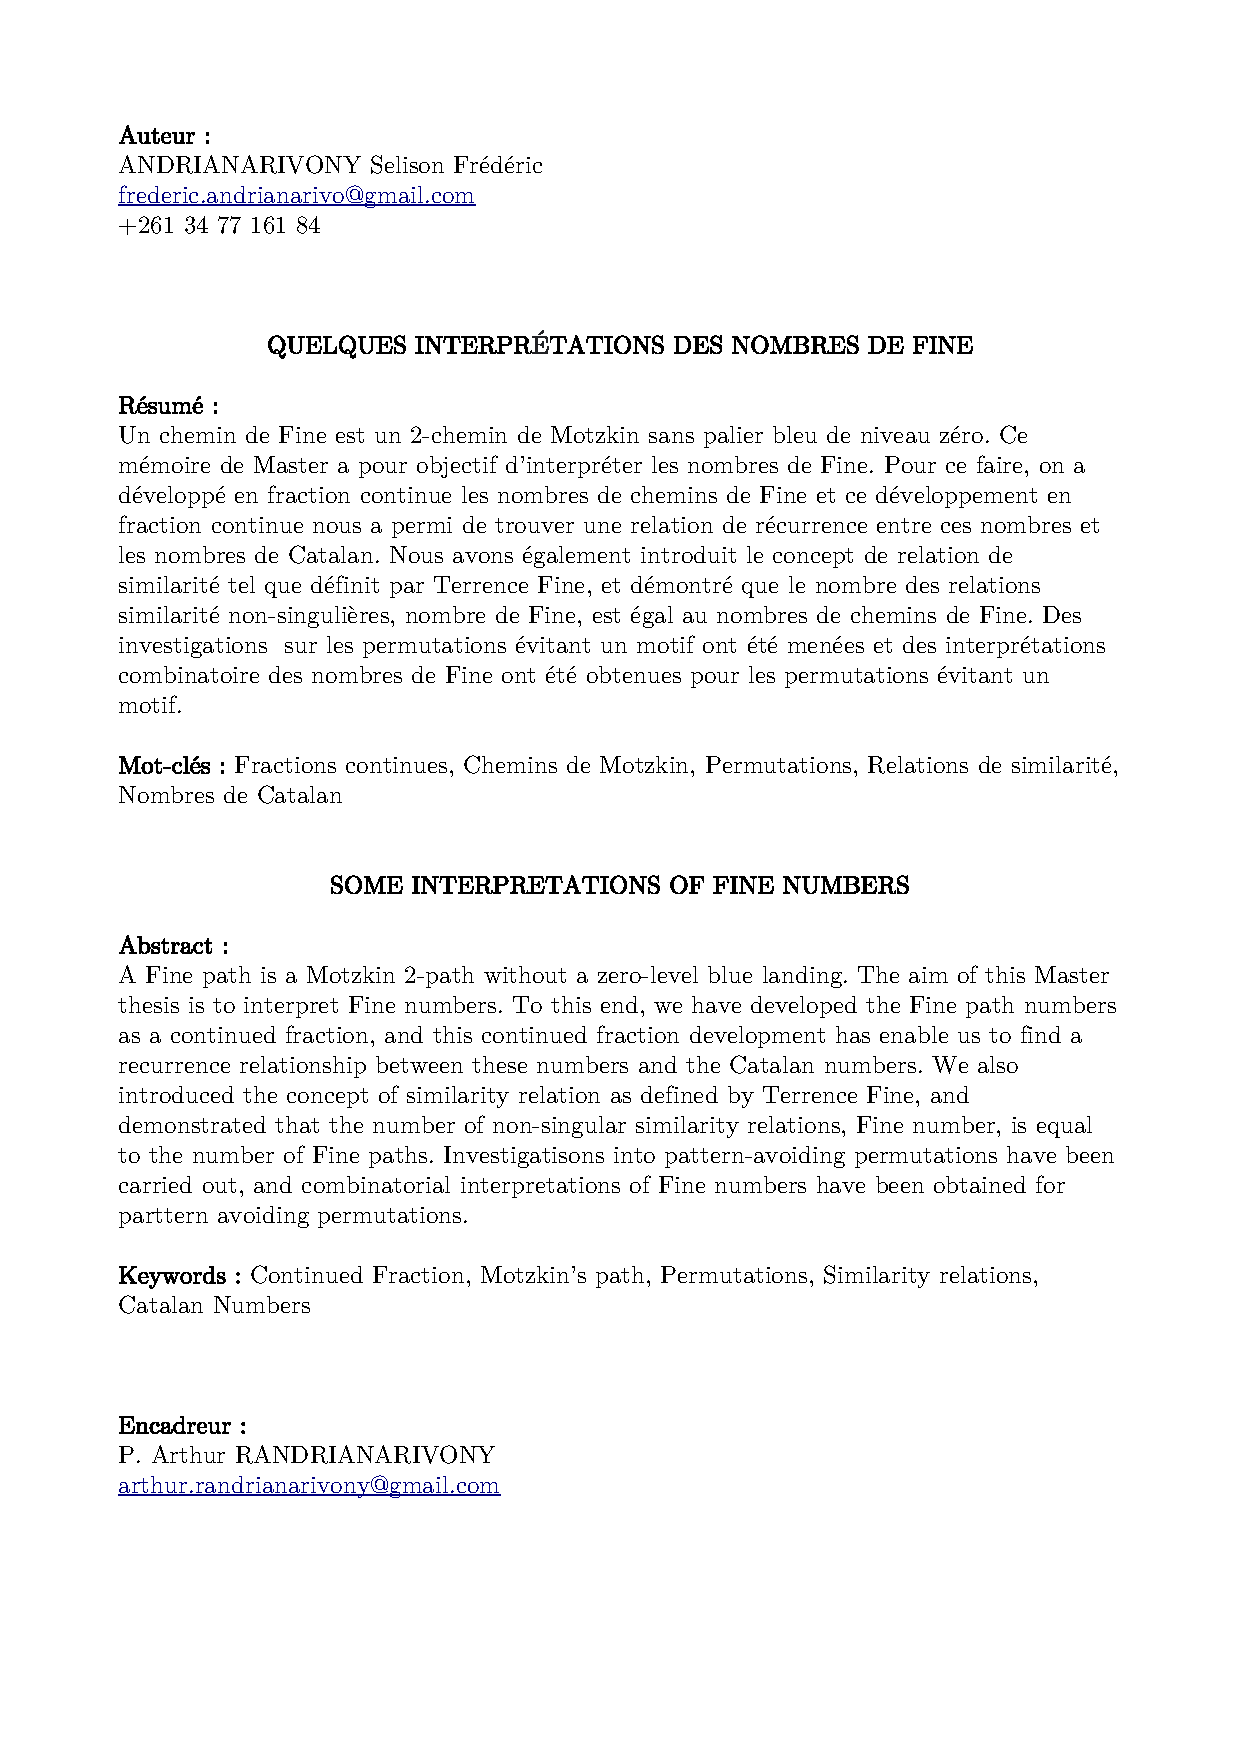
\includepdf[pages=-]{Summary.pdf}
\end{document}
